\subsection{The conjugate gradient method}

The conjugate gradient method is used to solve a general linear system
%
\begin{equation}
    \mathrm{A} \bm{x} = \bm{b},
\end{equation}
%
where \(\mathrm{A}\) is an \(N \times N\) symmetric, positive definite
matrix, and \(\bm{b}\) is an \(N \times 1\)
vector, and \(\bm{x}\) is the solution.
The algorithm is represented in Snippet~\ref{lst:cg}.

\begin{algorithm}[!hbt]
    \caption{The conjugate gradient method implementation of solving
        \(\mathrm{ A }\bm{ x } = \bm{ b }\).}
    \label{lst:cg}
    \begin{juliacode}
function solve!(logger, A, 𝐛, 𝐱₀=zeros(length(𝐛)); atol=eps(), maxiter=2000)
    𝐱ₙ = 𝐱₀
    𝐫ₙ = 𝐛 - A * 𝐱ₙ  # Initial residual, 𝐫₀
    𝐩ₙ = 𝐫ₙ  # Initial momentum, 𝐩₀
    for n in 0:maxiter
        if norm(𝐫ₙ) < atol
            setconverged!(logger)
            break
        end
        A𝐩ₙ = A * 𝐩ₙ  # Avoid duplicated computation
        αₙ = 𝐫ₙ ⋅ 𝐫ₙ / 𝐩ₙ ⋅ A𝐩ₙ  # `⋅` means dot product between two vectors
        𝐱ₙ₊₁ = 𝐱ₙ + αₙ * 𝐩ₙ
        𝐫ₙ₊₁ = 𝐫ₙ - αₙ * A𝐩ₙ
        βₙ = 𝐫ₙ₊₁ ⋅ 𝐫ₙ₊₁ / 𝐫ₙ ⋅ 𝐫ₙ
        𝐩ₙ₊₁ = 𝐫ₙ₊₁ + βₙ * 𝐩ₙ
        log!(logger, IterationStep(n, αₙ, βₙ, 𝐱ₙ, 𝐫ₙ, 𝐩ₙ))
        # Prepare for a new iteration
        𝐱ₙ, 𝐫ₙ, 𝐩ₙ = 𝐱ₙ₊₁, 𝐫ₙ₊₁, 𝐩ₙ₊₁
    end
    return 𝐱ₙ
end
    \end{juliacode}
\end{algorithm}


\subsection{Recap the question}

The problem to solve is
%
\begin{spreadlines}{2ex} % See https://tex.stackexchange.com/a/577172
    \begin{equation}
        \begin{dcases}
            \begin{aligned}
                \nabla^2 \phi(x, y) & = -\rho, & (x, y) \in \square;         \\
                \phi(x, y)          & = 0,     & (x, y) \in \partial\square; \\
                \phi(x, y)          & = 5,     & (x, y) \in \blacksquare;
            \end{aligned}
        \end{dcases}
    \end{equation}
\end{spreadlines}
%
where \(\square\) denotes the two-dimensional simulation box,
\(\partial\square\) denotes the boundary of the box,
and \(\blacksquare\) denotes the solid internal square.

First, we want to discretize the Laplacian operator \(\nabla^2\).
With grid spacing \(a\), the standard discretization for a square grid is
%
\begin{multline}\label{eq:del2phi}
    \nabla^2 \phi(x, y) =
    \frac{ 1 }{ a^2 } \bigl(\phi(x - a, y) - 2 \phi(x, y) + \phi(x + a, y)\bigr) +\\
    \frac{ 1 }{ a^2 } \bigl(\phi(x, y - a) - 2 \phi(x, y) + \phi(x, y + a)\bigr).
\end{multline}
%
We simplify Equation~\eqref{eq:del2phi} as
%
\begin{equation}\label{eq:del2phisim}
    \bigl(\nabla^2 \phi\bigr)_{i, j} = \frac{1}{a^2} \bigl(
    -4 \phi_{i, j} + \phi_{i+1, j} + \phi_{i-1, j} + \phi_{i, j-1} + \phi_{i, j+1}
    \bigr),
\end{equation}
%
for all \(i\) and \(j\),
where \(i\) and \(j\) label the \(x\) and \(y\) coordinates, respectively.
Equation~\eqref{eq:del2phi} is what we called the \emph{five-point stencil}
for the discretization of a Laplacian using central differences,
as shown in Figure~\ref{fig:stencil}.

% See https://tex.stackexchange.com/a/227247
\begin{figure}
    \centering
    \begin{tikzpicture}
        \draw[thick] (0,0) grid (4,4); % See https://tex.stackexchange.com/a/552215
        \stencilpt[red]{2,2}{i}  {$-4$};
        \stencilpt{1,2}{i-1}{$1$};
        \stencilpt{3,2}{i+1}{$1$};
        \stencilpt{2,1}{j-1}{$1$};
        \stencilpt{2,3}{j+1}{$1$};
        \draw
        (j-1) -- (i)
        (i)   -- (j+1)
        (i-1) -- (i)
        (i)   -- (i+1);
    \end{tikzpicture}
    \caption{The \href{https://en.wikipedia.org/wiki/Five-point_stencil}{five-point stencil}
        for the discretization of a Laplacian using central differences.}
    \label{fig:stencil}
\end{figure}


By starting at the upper left corner and traversing in the \(y\)-direction first, and
subsequently in the \(x\)-direction---the lexicographical ordering---we get the following
system of equations:
%
\begin{align}
    \bigl(\nabla^2 \phi\bigr)_{i, j+1}   & = \frac{1}{a^2} (
    \phi_{i, j} - 4\phi_{i, j+1} + \phi_{i, j+2} + \phi_{i+1, j+1} + \phi_{i-1, j+1}
    ),                                                       \\
    \bigl(\nabla^2 \phi\bigr)_{i+1, j}   & = \frac{1}{a^2} (
    \phi_{i, j} - 4\phi_{i+1, j} + \phi_{i+1, j+1} + \phi_{i+1, j-1} + \phi_{i+2, j}
    ),                                                       \\
    \bigl(\nabla^2 \phi\bigr)_{i+1, j+1} & = \frac{1}{a^2} (
    \phi_{i, j+1} + \phi_{i+1, j} - 4\phi_{i+1, j+1} + \phi_{i+1, j+2} + \phi_{i+2, j+1}
    ),                                                       \\
    \shortvdotswithin{=} % See https://tex.stackexchange.com/a/67196
    \bigl(\nabla^2 \phi\bigr)_{i-1, j-2} & = \frac{1}{a^2} (
    \phi_{i-1, j-3} + \phi_{i, j-2} + \phi_{i-2, j-2} - 4\phi_{i-1, j-2} + \phi_{i-1, j-1}
    ),                                                       \\
    \bigl(\nabla^2 \phi\bigr)_{i-1, j-1} & = \frac{1}{a^2} (
    \phi_{i-1, j} + \phi_{i-1, j-2} + \phi_{i, j-1} + \phi_{i-2, j-1} - 4\phi_{i-1, j-1}
    ).\label{eq:delend}
\end{align}
%
Here we apply the periodic boundary condition
%
\begin{align}
    \phi(x + (N-1)a, y) & = \phi(x - a, y), \\
    \phi(x, y + (N-1)a) & = \phi(x, y - a).
\end{align}

\begin{figure}[!hbt]
    \centering
    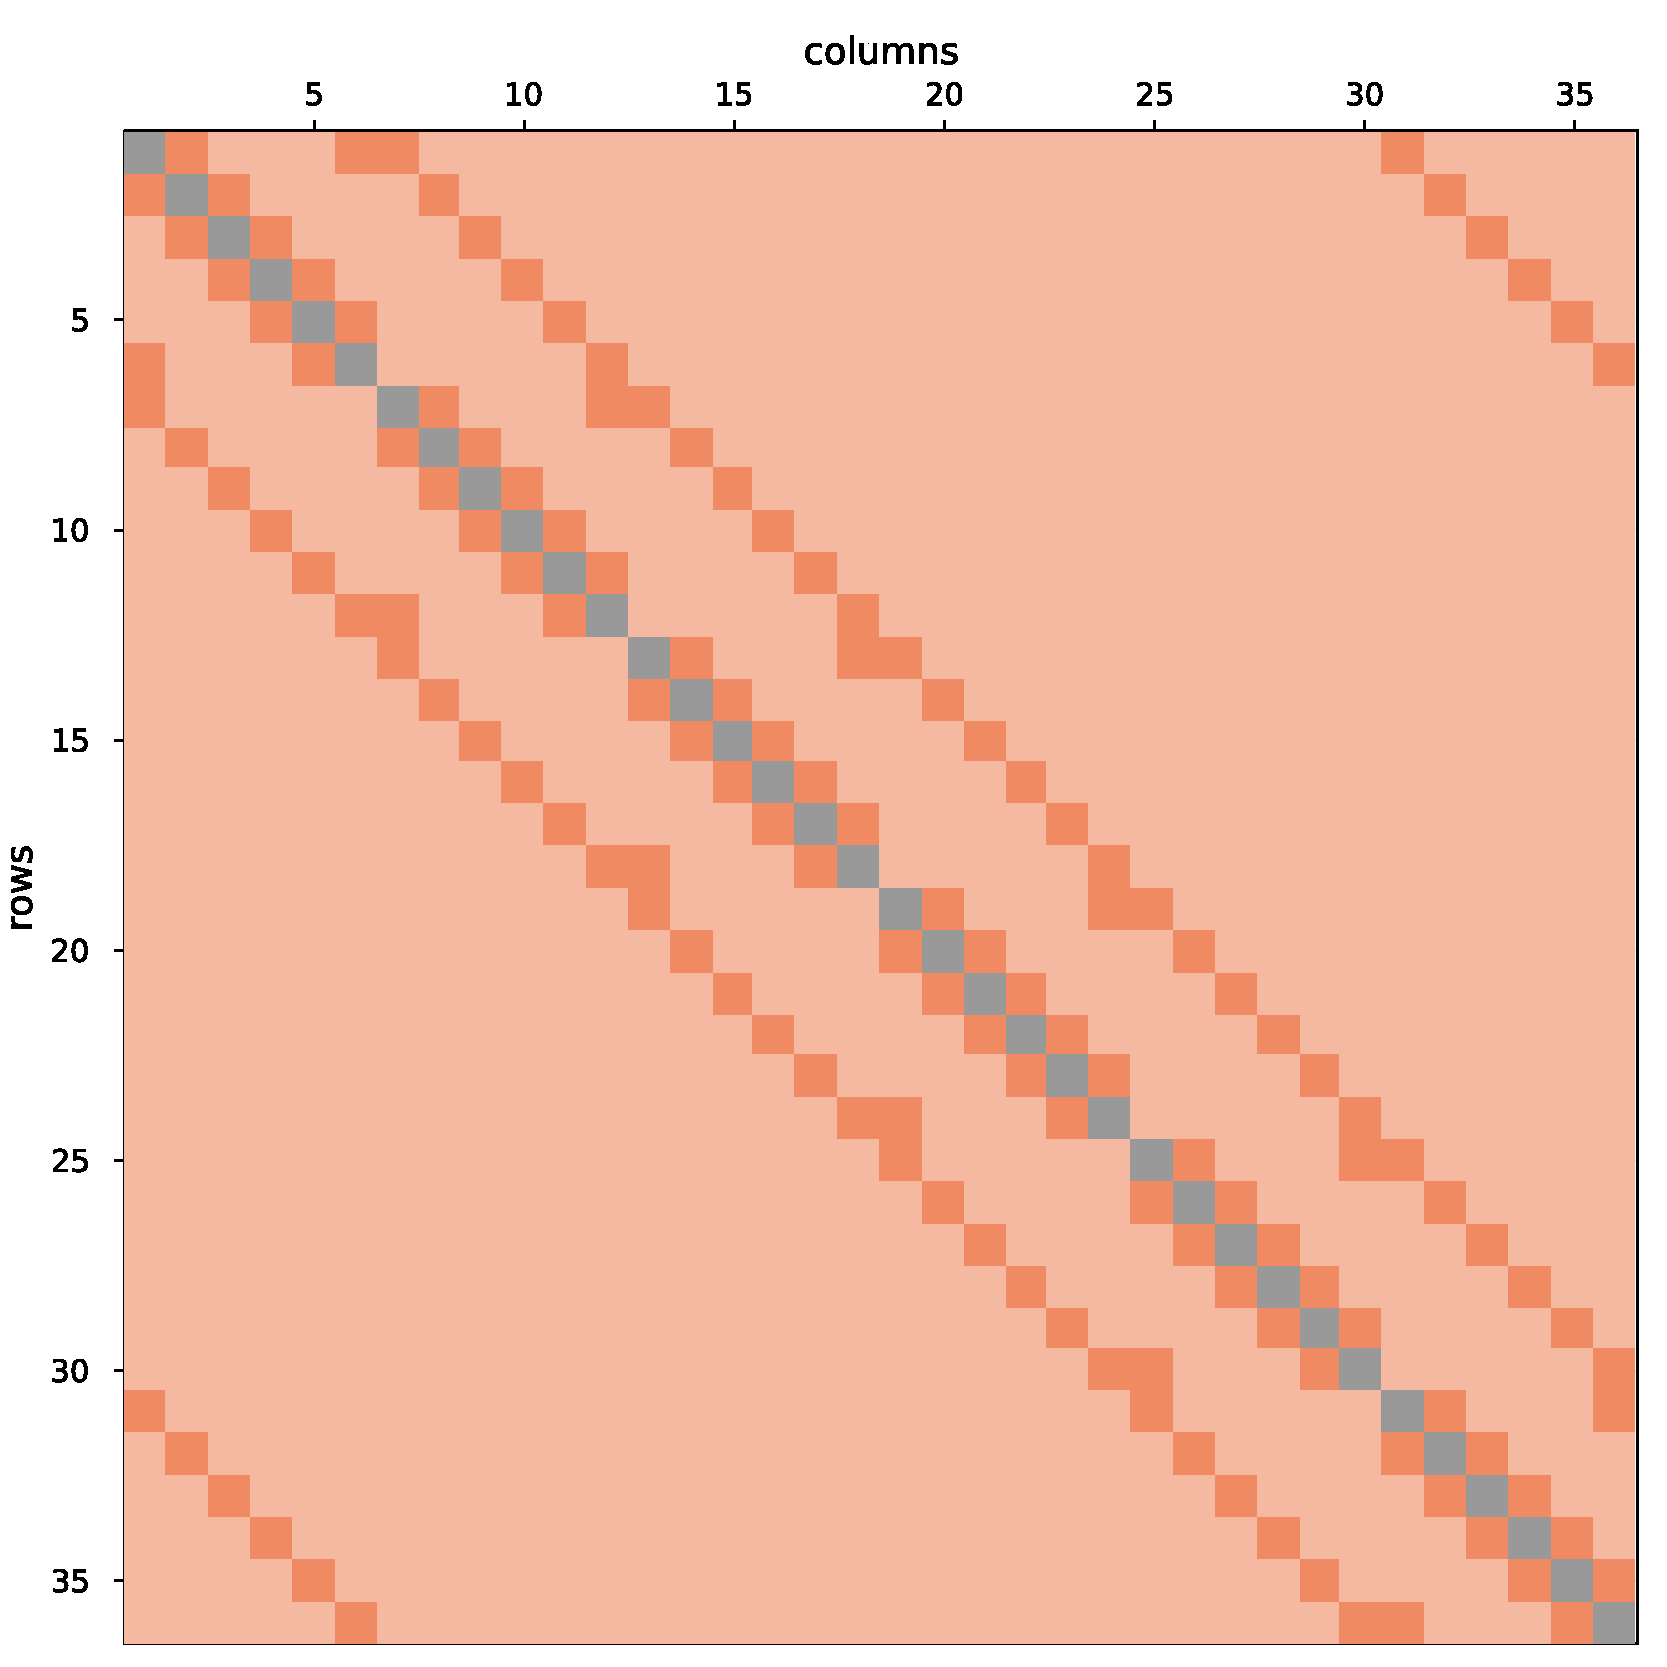
\includegraphics[width=0.8\textwidth]{laplacian}
    \caption{The heatmap of the discrete Laplacian with \(N = 6\), and hence
        the Laplacian matrix is of size \(36 \times 36\).
        The color gray denotes \(4\) on the diagonal of the matrix, and
        the color red denotes \(-1\), and the background light red
        denotes the zeros.
        As we can observe, the discrete Laplacian is a sparse, symmetric matrix.}
    \label{fig:laplacian}
\end{figure}

We can simplify Equations~\eqref{eq:del2phisim} to~\eqref{eq:delend} into a matrix
representation, i.e., the discrete Laplacian representation:
%
\begin{equation}\label{eq:Axb}
    \begin{split}
        -\bm{\rho} &= \frac{ 1 }{ a^2 } \begin{bsmallmatrix}
            -4     & 1      & 0      & \cdots & 0      & 1      & 1      & 0      & \cdots & 0      & 0      & \cdots & 1      & \cdots & 0      & 0      \\
            1      & -4     & 1      & \cdots & 0      & 0      & 0      & 1      & \cdots & 1      & 0      & \cdots & 0      & \cdots & 0      & 0      \\
            \vdots & \vdots & \vdots & \ddots & \vdots & \vdots & \vdots & \vdots & \ddots & \vdots & \vdots & \ddots & \vdots & \ddots & \vdots & \vdots \\
            1      & 0      & 0      & \cdots & 0      & 0      & -4     & 1      & \cdots & 1      & 1      & \cdots & 0      & \cdots & 0      & 0      \\
            0      & 1      & 0      & \cdots & 0      & 0      & 1      & -4     & \cdots & 0      & 0      & \cdots & 0      & \cdots & 0      & 0      \\
            \vdots & \vdots & \vdots & \ddots & \vdots & \vdots & \vdots & \vdots & \ddots & \vdots & \vdots & \ddots & \vdots & \ddots & \vdots & \vdots \\
            0      & 0      & 0      & \cdots & 1      & 0      & 0      & 0      & \cdots & 0      & 0      & \cdots & 0      & \cdots & -4     & 1      \\
            0      & 0      & 0      & \cdots & 0      & 1      & 0      & 0      & \cdots & 0      & 0      & \cdots & 1      & \cdots & 1      & -4
        \end{bsmallmatrix}
        \begin{bsmallmatrix}
            \phi_{0, 0} \\
            \phi_{0, 1} \\
            \phi_{0, 2} \\
            \vdots \\
            \phi_{0, N-2} = \phi_{0, -2} \\
            \phi_{0, N-1} = \phi_{0, -1} \\
            \phi_{1, 0} \\
            \phi_{1, 1} \\
            \vdots \\
            \phi_{1, N-1} = \phi_{1, -1} \\
            \phi_{2, 0} \\
            \vdots \\
            \phi_{N-1, 0} = \phi_{-1, 0} \\
            \vdots \\
            \phi_{N-1, N-2} = \phi_{-1, -2} \\
            \phi_{N-1, N-1} = \phi_{-1, -1}
        \end{bsmallmatrix} \\
        &= \mathrm{ A } \bm{\phi},
    \end{split}
\end{equation}
%
where \(\mathrm{ A }\) (the discrete Laplacian) is a \(N^2 \times N^2\) matrix,
and \(\bm{\phi}\) and \(\bm{\rho}\) are \(N^2 \times 1\) vectors.
Notice that the structure of the coefficient matrix \(\mathrm{ A }\) is completely dictated
by the way that the basis is ordered.
The non-zero elements in the coefficient matrix are markers for which \(\phi\) is coupled
with each other.

However, there is one trick in Equation~\eqref{eq:poisson}.
If we following the notation by Equation~\eqref{eq:poisson}, the discrete Laplacian
\(\mathrm{ A }\) is not a positive definite matrix.
However, to use the conjugate gradient method, we need \(\mathrm{ A }\) to be a
positive definite matrix. We still have some work to do.

By our formulation, \(\mathrm{ A }\) is a symmetric matrix.
To judge whether a symmetric matrix is a positive definite matrix, we use the
Sylvester's criterion:
%
\begin{theorem}[Sylvester]
    A symmetric matrix \(\mathrm{ A }\) is positive definite if and only if all its
    leading principal minors are positive.
\end{theorem}
%
Obviously, \(\mathrm{ A }\) in Equation~\eqref{eq:Axb} does not satisfy this criterion.
Fortuantely, if we rewrite Equation~\eqref{eq:poisson} as
%
\begin{equation}\label{eq:poissoncorrected}
    -\nabla^2 \phi = \rho,
\end{equation}
%
then all of the elements of \(\mathrm{ A }\) in Equation~\eqref{eq:Axb} are negated.
And amazingly, \(\mathrm{ A }\) is now a positive definite matrix!
So the actual problem we are solving is
%
\begin{equation}
    \mathrm{ A }' \bm{\phi} = \bm{\rho},
\end{equation}
%
where \(\mathrm{ A }' = -\mathrm{ A }\).

We can also prove that each row (column) of the matrix sums to \(0\) by
translational symmetry. Therefore, the rules for numerically generating
the matrix are\footnotemark{}:
%
\begin{itemize}
    \item All main diagonal elements are \(4\).
    \item The superdiagonal elements (\(k = 1\)) are either \(0\) or \(-1\).
    \item The \((N-1)\)th diagonal elements are either \(0\) or \(-1\).
    \item The \(N\)th diagonal elements are all \(-1\).
    \item The \((N(N - 1))\)th diagonal elements are all \(-1\).
\end{itemize}
%
\footnotetext{The general term for any diagonal going top-left to bottom-right
    direction is \(k\)-diagonal where \(k\) is an offset from the main diagonal.}

The heatmap of a discrete Laplacian with \(N = 6\) is plotted in Figure~\ref{fig:laplacian}.
The corresponding Laplacian matrix is of size \(36 \times 36\).
Obviously, the discrete Laplacian is a sparse matrix.
We could use sparse matrix algorithms or just use Equation~\eqref{eq:del2phi} in the actual
implementation.
In vector \(\bm{\phi}\), we order the \(\phi\)'s in \(y\)-direction first and then
\(x\)-direction, as stated above.

For a rectangle box of size \(M \times N\), the linear index \(n\) of point \((i, j)\)
on the grid is
%
\begin{equation}\label{eq:nij}
    n = N i + j,
\end{equation}
%
in the \(y\)-direction first indexing order, where \(n = 1\), \(\ldots\), \(N^2\).
And since \(x = a i = i\), \(y = a j = j\), Equation~\eqref{eq:nij} can be rewritten as
%
\begin{equation}
    n = N x + y.
\end{equation}
%
We draw a schematic plot of the system with \(L = 32\) (\(N = 33\)) for simplicity in
Figure~\ref{fig:grid}, where you can observe this relation.
In the iterative solver for Equation~\eqref{eq:Axb},
the initial vector \(\bm{\rho}(0)\) has \(\rho(0)_a = -20\) and \(\rho(0)_b = -20\),
and zero everywhere else,
where \(a\) and \(b\) are the linear indices of the two charges.
And the initial vector \(\bm{\phi}(0)\) has \(5\) in the components corresponding to
the points in the solid square, and has zero in the components corresponding to
the boundary of the region while having non-zero values everywhere else.
The solid square in the interior has length \(L/4\) and
its center is at \((x, y) = (5L/8, 3L/4)\).
The point charges are at \((L/4, L/8)\) and \((3L/4, L/8)\).

\begin{figure}[!hbt]
    \centering
    \begin{subfigure}[t]{0.49\linewidth}
        \centering
        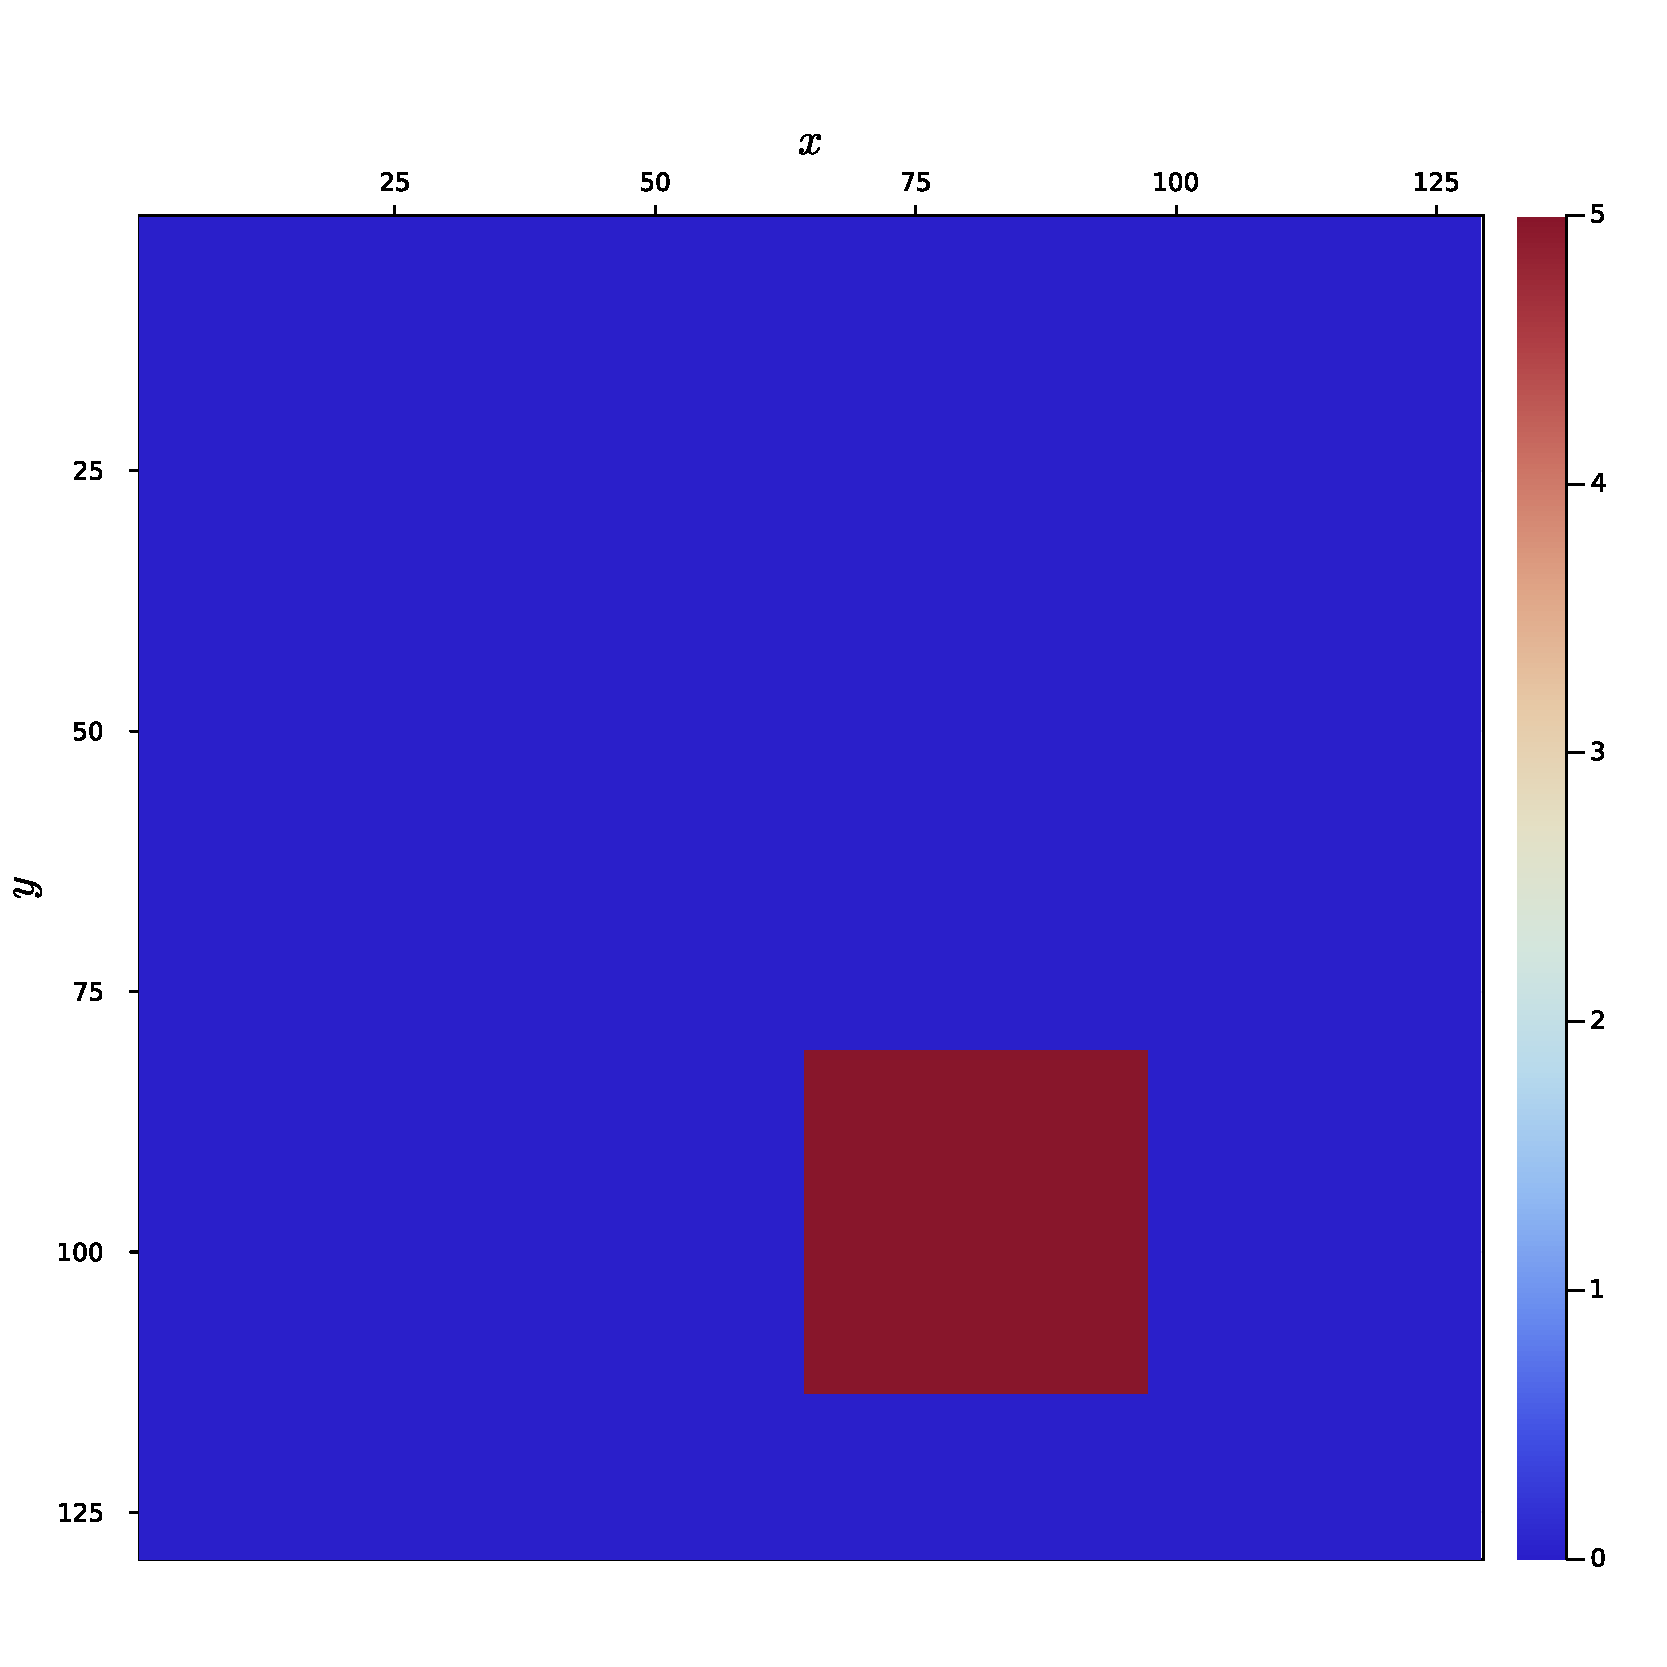
\includegraphics[width=\linewidth]{phi0_heatmap}
        \caption{\label{fig:t0:a}}
    \end{subfigure}
    \hfill
    \begin{subfigure}[t]{0.49\linewidth}
        \centering
        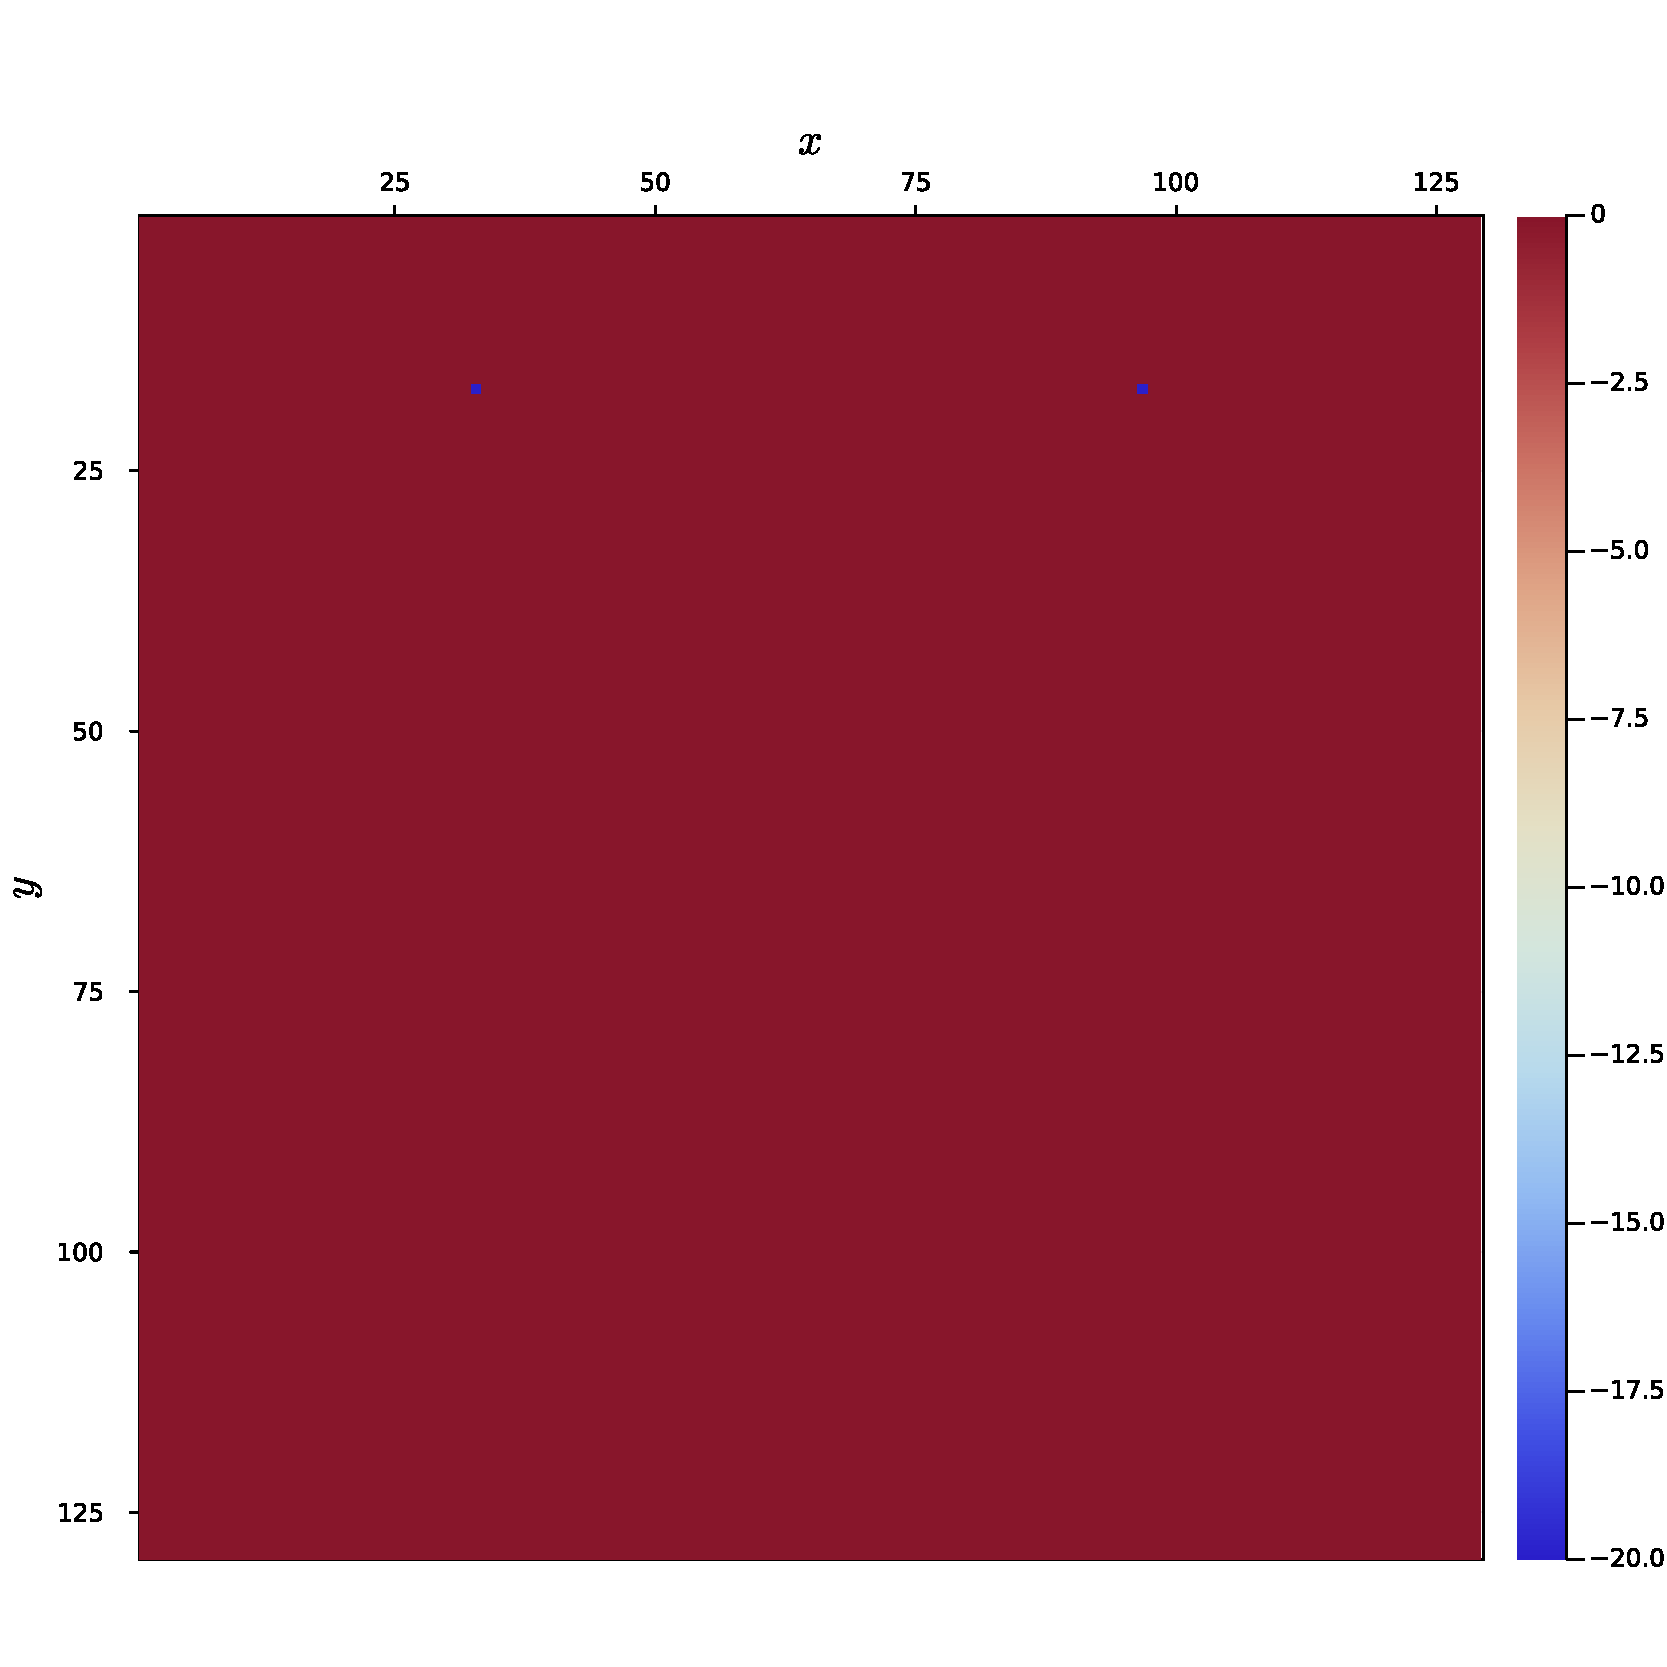
\includegraphics[width=\linewidth]{rho_heatmap}
        \caption{\label{fig:t0:b}}
    \end{subfigure}
    \caption{The heatmaps of the initial values (\protect\subref{fig:t0:a}) \(\bm{\phi}(0)\)
        and (\protect\subref{fig:t0:b}) charge density \(\bm{\rho}\)
        with \(L = 128\) (\(N = 129\)).}
    \label{fig:status}
\end{figure}

One thing to notice is that if we want to plot a heatmap of
the matrix according to its layout in Julia, its columns are plotted in the
horizontal direction (the \(x\) direction in Figure~\ref{fig:grid}),
and its rows are plotted in the vertical direction
(the \(y\) direction in Figure~\ref{fig:grid}).
So we need to transpose its elements when indexing the matrix.
Also, since \(x\) and \(y\) span from \(0\) to \(L\), the actual matrix is of size
\(N \times N = (L + 1) \times (L + 1)\), as shown in Figure~\ref{fig:grid}.
So when indexing the elements in the internal square and the point charges,
we need to subtract \(1\) from our matrix's size and multiply it by the corresponding
fraction, then add \(1\) back to obtain the correct index of an element in the
specific area.
Figures~\ref{fig:t0:a} and~\ref{fig:t0:b} show the heatmaps of
\(\bm{\phi}(0)\) and \(\bm{\rho}\) with \(L = 128\) (i.e., \(N = 129\)).

We benefit from using the configuration shown in Figure~\ref{fig:grid} that it follows
Julia's matrix column-major order for storing multidimensional arrays in linear storage, such
as random access memory.
Therefore, we could just \code{reshape} the \(N^2 \times 1\) \(\bm{\phi}\) vector
(solution) obtained into an \(N \times N\) matrix for easier plotting,
as shown in Snippet~\ref{lst:reshape}.
%
\begin{algorithm}
    \caption{Reshape the \(N^2 \times 1\) \(\bm{\phi}\) vector
        (solution) obtained into an \(N \times N\) \(\phi(x, y)\) matrix.}
    \label{lst:reshape}
    \begin{juliacode}
ϕ = reshape(𝛟, N, N)
    \end{juliacode}
\end{algorithm}
